\documentclass[a4paper]{report}

\usepackage{generalsnips}
\usepackage{calculussnips}
\usepackage[margin = 0.80in]{geometry}
\usepackage{pdfpages}
\usepackage[spanish]{babel}
\usepackage{amsmath}
\usepackage{amsthm}
\usepackage[utf8]{inputenc}
\usepackage{titlesec}
\usepackage{xpatch}
\usepackage{fancyhdr}
\usepackage{tikz}
\usepackage{float}
\usepackage{multicol}
\usepackage{wrapfig}
\usepackage{blindtext}
\usepackage{array}
\usepackage{enumitem}
\usepackage{url}
\usepackage{breakurl}
\usepackage{hyperref}
\decimalpoint
\begin{document}
\sloppy
\begin{titlepage}

    \title{}
    
\end{titlepage}


\begin{titlepage}
    \begin{center}
        \thispagestyle{empty}
        \renewcommand{\headrulewidth}{0pt}
        \renewcommand{\footrulewidth}{0pt}
        
        \begin{tabular}{ p{0.5\textwidth}p{0.5\textwidth} }
            \begin{flushleft}
                Facultad de Ciencias Económicas \\
                Universidad Francisco Marroquín \\
                Administración Financiera I \\ 
                Catedrático: Ana Del Carmen Muñoz Del Valle \\ 
                Auxiliar: Edwin Adalberto Calderón Cárdenas \\
                Guatemala \\
                07 de septiembre 2020 \\ 
            \end{flushleft}
            &
            \begin{flushright}
                
\includegraphics[width=0.5\textwidth]{ufmlogo.png} \\ 
            \end{flushright} \\ 
        \end{tabular}
        
            
        \cfoot{} % this is to remove the page number
        \vspace*{7cm}
        {
            \Huge Parte Teórica Parcial \#1 - Administración Financiera I
        }
 
        \vspace{1.5cm}

 
        \vfill
             
        \vspace{0.8cm}
        
        
        \begin{flushleft}
            \begin{tabular}{ ll }
                David Corzo      & 20190432 \\
                Daniel Cabrera   & 20190069 \\
            \end{tabular}
        \end{flushleft}     
    \end{center}
\end{titlepage}

%%%%%%%%%%%%%%%%%%%%%%%%%%%%%%%%%%%%%%%%%%%%%%%%%%%%%%%%%%%%%%%%%%%%%%%%%%%
\section{Introducción}
Desde su legalización en algunos estados de Estados Unidos para uso recreativo, se ha cuestionado mucho el daño que el Cannabis representa para el ser humano a costa de sus efectos “placenteros”, especialmente en los adolescentes, los cuales están más dispuestos a consumirla que generaciones pasadas. \par 
\begin{quote}
    La marihuana es la droga psicotrópica más utilizada en los Estados Unidos, después del alcohol. En 2018, más de 11,8 millones de adultos jóvenes informaron haber consumido marihuana en el último año. Su uso es más frecuente entre los hombres que entre las mujeres. En 2019, el 11,8\% de los estudiantes de octavo grado informó haber consumido marihuana el año pasado y el 6,6\% el mes pasado (uso actual). Entre los estudiantes de décimo grado, el 28,8\% había consumido marihuana el año pasado y el 18,4\% el mes pasado. Las tasas de consumo entre los estudiantes de 12º grado fueron aún más altas: el 35,7\% había consumido marihuana durante el año anterior a la encuesta y el 22,3\% la había utilizado en el último mes; El 6,4\% dijo que consumía marihuana a diario o casi a diario. [4]
\end{quote}
En 2014, se publicaron hallazgos de neuroimagen, neurocognitivos y preclínicos sobre los efectos del cannabis en el cerebro de los adolescentes. Entre sus conclusiones, se mencionó la existencia de ``desventajas neurocognitivas del consumo de marihuana en los dominios de la atención y la memoria que persisten más allá de la abstinencia, sino que sugieren posibles alteraciones macroestructurales del cerebro [...]'' [3] presentadas en el libro Monitoring the future: National results on adolescent drug use: Overview of key findings, 2000 por Lloyd Johnston, Patrick M O´Malley y Jerald G Bachman.
Sin embargo, por su parte el alcohol a pesar de su mayor popularidad e incontables estudios describiendo sus efectos negativos a corto y largo plazo, es tomado por la sociedad como un vicio común y mucho más aceptable que su competidor. \par 

Esto nos inspiró a realizar nuestro propio estudio enfocándonos en el desempeño mental de los jóvenes bajo los efectos de estas sustancias. Específicamente, si alguien bajo los efectos del alcohol podría tener un mejor rendimiento en una prueba matemática difícil, que haciendo la misma prueba bajo los efectos del cannabis. Para esto les dimos a los participantes del experimento un té de cannabis de 250 ml que aproximadamente contenía 2.5 gr de la planta (de acuerdo al listado de ingredientes de esta bebida en Wikipedia) y un shot de 30 ml de Vodka, el equivalente a 12 ml de alcohol. 

    
    
\section{Descripción de la investigación}
De un estudio fueron obtenidos resultados de pruebas matemáticas después de ingerir alcohol y después de ingerir cannabis. La hipótesis de investigación indica que el alcohol afecta negativamente en un nivel mayor el desempeño mental en comparación con el cannabis.
A continuación se presentan las puntuaciones obtenidas en el examen matemático después de ingerir alcohol y después de ingerir cannabis.

\section{Prueba de hipótesis}

\begin{itemize}
    \item \textbf{Hipótesis nula:} el resultado promedio de los exámenes realizados después de consumir alcohol será más alto o igual que el de cannabis
    \item \textbf{Hipótesis alternativa:} el resultado promedio de los exámenes realizados después de consumir alcohol será más bajo que el de cannabis.
\end{itemize}

\begin{center}
    {
        \begin{tabular}{ |l|c| }
            \hline
                \multicolumn{2}{|c|}{\textbf{Prueba matemática después de alcohol}} 
            \\ 
            \hline
                Media$_1$ & 26.55 \\ 
            \hline
                Desviación estándar$_1$ & 7.316822906 \\ 
            \hline
                Varianza de la muestra$_1$ & 53.53589744 \\ 
            \hline
                $n_1$ & 40 \\ 
            \hline
        \end{tabular}
    }
    {
        \begin{tabular}{ |l|c| }
            \hline
                \multicolumn{2}{|c|}{\textbf{Prueba matemática después de cannabis}} 
            \\ 
            \hline
                Media$_2$ & 29.5 \\ 
            \hline
                Desviación estándar$_2$ & 6.606135454 \\ 
            \hline
                Varianza de la muestra$_2$ & 43.64102564 \\ 
            \hline
                $n_2$ & 40 \\ 
            \hline
        \end{tabular}
    }
\end{center}

\begin{enumerate}
    \item \textbf{Establecer el parámetro de interés:} $\mu_1-\mu_2$ 
    \item \textbf{Establecer hipótesis:}
        \begin{center}
           \begin{align*}
               H_0: \mu_1 \geq \mu_2 \\ 
               H_a: \mu_1 < \mu_2 \\
           \end{align*}
        \end{center}
    
    \item \textbf{Establecer significancia:} $\alpha = 0.05$
    \item \textbf{Estadístico de prueba:}
        Tomando como referencia la fórmula de distribución T: 
        \[
          t = \frac{
              \bar{x_1}-\bar{x_2}-D_0
            }{
                \sqrt{
                    \cfrac{s_1^2}{n_1} + \cfrac{s_2^2}{n_2}
                }
            }
        \] Sustituyendo los datos: 
        \begin{center}
           \begin{align*}
                t = \frac{
                    26.55-29.50
                    -0
                }{
                    \sqrt{
                        \cfrac{53.5358974358975}{40} + \cfrac{43.6410256410256}{40}
                    }
                } = -1.892650569
           \end{align*}
        \end{center}
        Ahora determinar los grados de libertad: 
        \[
            gl = \left\lfloor  \frac{
                \p{\cfrac{s_1^2}{n_1}+\cfrac{s_2^2}{n_2}}^2 
            }{
                \cfrac{1}{n_1-1} \p{\cfrac{s_1^2}{n_1}}^2 + \cfrac{1}{n_2-1}\p{\cfrac{s_2^2}{n_2}}^2   
            } \right\rfloor  
        \]
        Sustituyendo los datos: 
        \begin{center}
        \begin{align*}
                gl = \left\lfloor 
                    \frac{
                        \p{\cfrac{53.5358974358975}{40}+\cfrac{43.6410256410256}{40}}^2 
                    }{
                        \cfrac{1}{40-1} \p{\cfrac{53.5358974358975}{40}}^2 + \cfrac{1}{40-1}\p{\cfrac{43.6410256410256}{40}}^2   
                    } 
                \right\rfloor  = \left\lfloor 77.19882 \right\rfloor  = 77
        \end{align*}
        \end{center}
        
    \item \textbf{Establecer criterio de rechazo:} $\displaystyle t_{\text{crít.}} = -1.665$. Rechazar $H_0$ si: $t \leq t_{\text{crít.}}$.
        \begin{figure}[H]
            \centering
            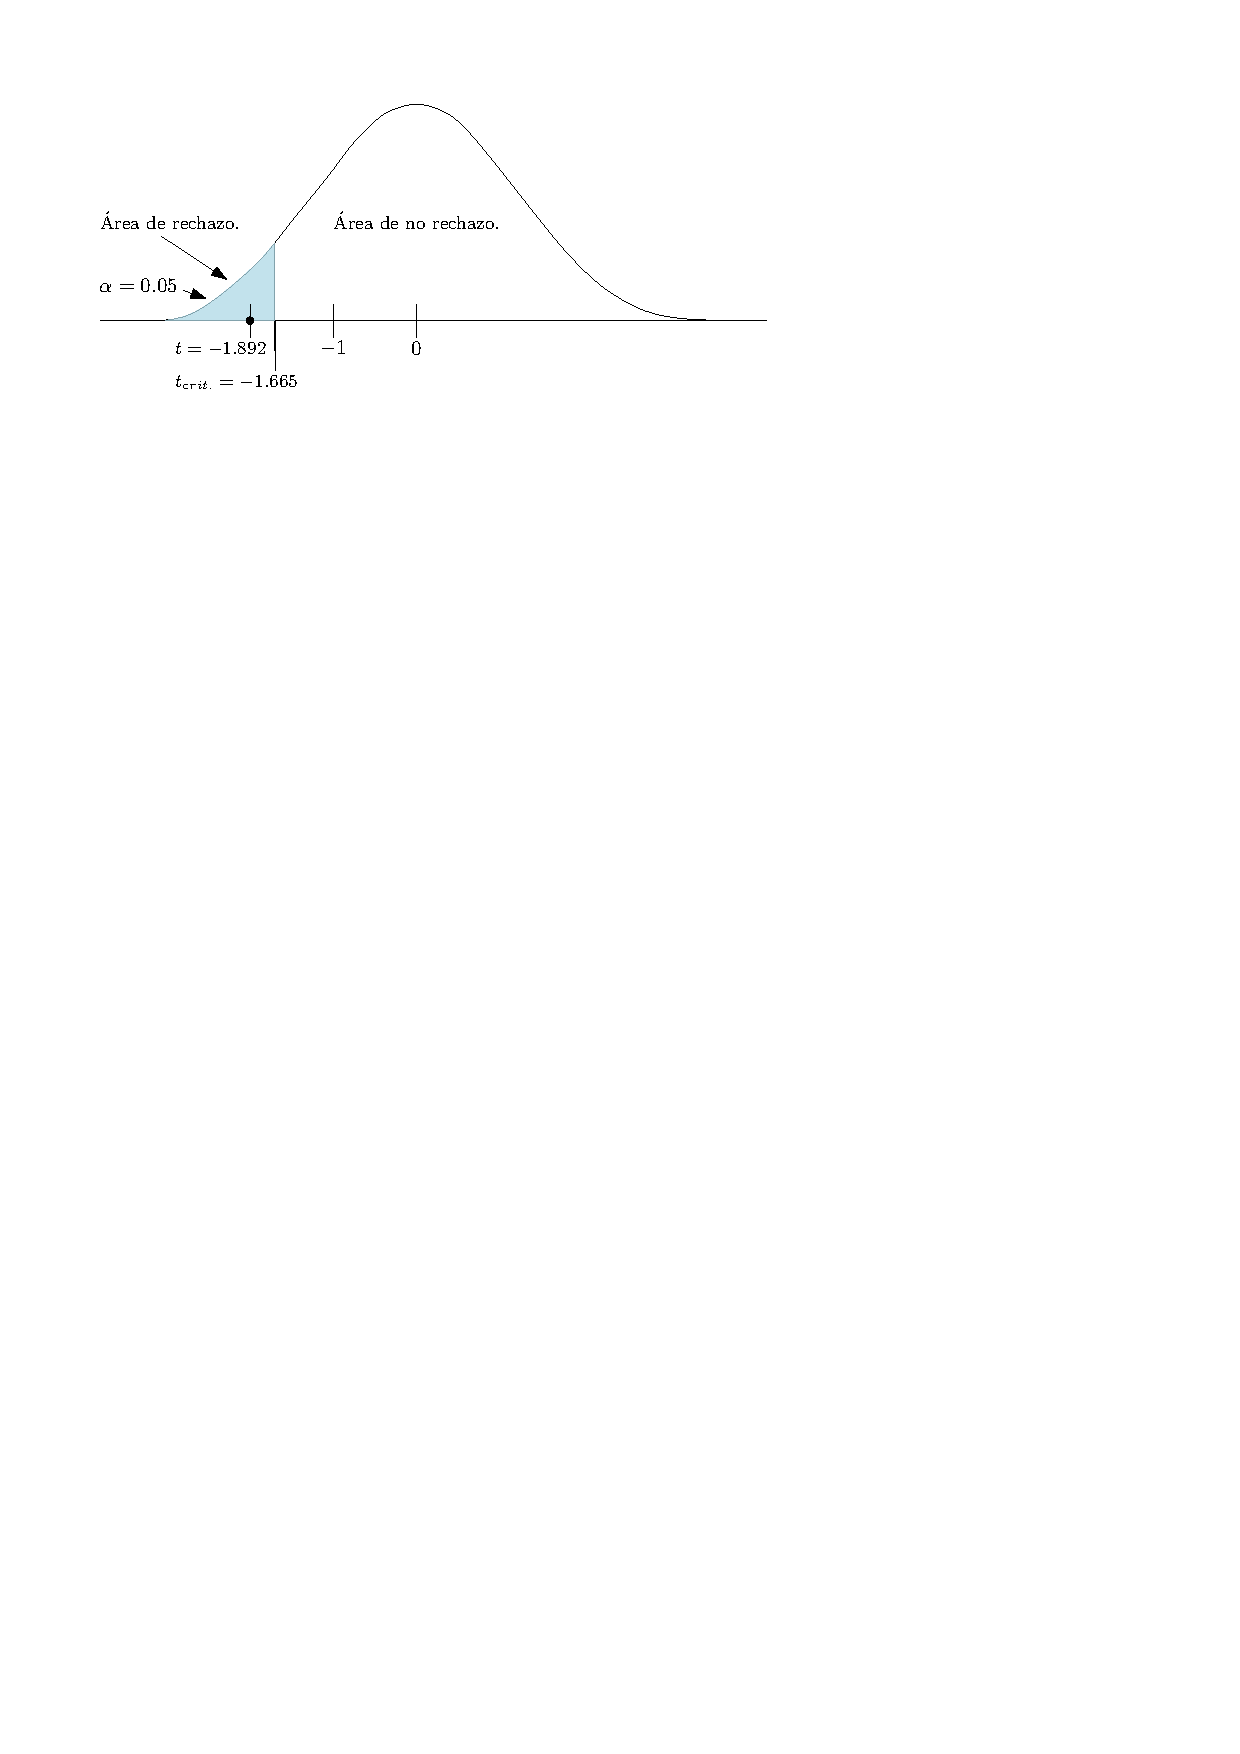
\includegraphics[width=\textwidth]{onetail.pdf}
        \end{figure}

    \item \textbf{Conclusión:} Con una significancia de $\alpha=0.05$ y una muestra de 40, hay suficiente evidencia para rechazar la hipótesis nula y podemos afirmar que el desempeño mental es menor al consumir alcohol que al consumir té de cannabis.
\end{enumerate}

\section{Justificación del tamaño de muestra}
Elegimos $n=40$ basándonos en lo mencionado en el libro: ``Se recomienda, siempre que sea posible, usar muestras del mismo tamaño, $n_1 = n_2$. Los procedimientos aquí presentados para estimaciones por intervalo y pruebas de hipótesis son sólidos y pueden usarse con muestras relativamente pequeñas. En la mayor parte de las aplicaciones con muestras iguales o casi del mismo tamaño, y de manera que el tamaño total de la muestra, $n_1 + n_2$, sea por lo menos 20, se esperan muy buenos resultados aun cuando las poblaciones no sean normales.''[1] \& ``En la mayor parte de las aplicaciones de estimaciones por intervalo y de pruebas de hipótesis presentadas en esta sección, las muestras aleatorias con $n_1 \geq 30$ y $n_2 \geq 30$ se consideran adecuadas''[2]

\subsection{Datos de la muestra}
De una población total de 139 personas, se seleccionaron 40 aleatoriamente, cada una de las personas había sido filtrada para asegurar los siguientes criterios: 
\begin{itemize}
    \item No hayan probado marihuana.
    \item No fuman extensamente, es decir: \emph{light smokers}, \emph{non-smokers}.
    \item No son alcohólicos.
\end{itemize}

\begin{center}
    \begin{tabular}{ |p{0.7cm}|p{0.7cm}|p{0.7cm}|p{0.7cm}| }
        \hline
            \multicolumn{4}{|c|}{P. después de alcohol } \\
        \hline
            30 & 22 & 27 & 29  \\
            22 & 28 & 24 & 23  \\
            39 & 23 & 26 & 34  \\
            31 & 25 & 37 & 9   \\
            39 & 36 & 26 & 35  \\
            20 & 23 & 16 & 19  \\
            24 & 36 & 29 & 24  \\
            36 & 11 & 13 & 26  \\
            33 & 23 & 26 & 24  \\
            33 & 32 & 20 & 29  \\
        \hline
    \end{tabular}
    \begin{tabular}{ |p{0.7cm}|p{0.7cm}|p{0.7cm}|p{0.7cm}| }
        \hline
        \multicolumn{4}{|c|}{ P. después de marihuana} \\ 
         
        \hline
            14 & 28 & 30 & 36 \\
            26 & 33 & 31 & 25 \\
            37 & 29 & 38 & 34 \\
            31 & 25 & 35 & 15 \\
            40 & 35 & 27 & 35 \\
            29 & 28 & 25 & 20 \\
            32 & 39 & 33 & 27 \\
            37 & 12 & 20 & 30 \\
            31 & 30 & 26 & 31 \\
            35 & 35 & 25 & 31 \\
        \hline
    \end{tabular}
\end{center}

\section*{Bibliografía}
\begin{enumerate}[label={[\arabic*]}]
    \item David R. Anderson \& Dennis J. Sweeney \& Thomas A. Williams. Estadística para administración y economía, pg. 412 cap. 10. 11$^{\text{va}}$ edición.
    \item David R. Anderson \& Dennis J. Sweeney \& Thomas A. Williams. Estadística para administración y economía, pg. 419 cap. 10. 11$^{\text{va}}$ edición.
    \item Jacobus, J., \& Tapert, S. F. (2014). Effects of Cannabis on the Adolescent Brain. Current pharmaceutical design, 20(13), 2186-2193.
    \item NIDA. (2020, abril 8). What is the scope of marijuana use in the United States? National Institute on Drug Abuse. \burl{https://www.drugabuse.gov/publications/research-reports/marijuana/what-scope-marijuana-use-in-united-states}
\end{enumerate}
%%%%%%%%%%%%%%%%%%%%%%%%%%%%%%%%%%%%%%%%%%%%%%%%%%%%%%%%%%%%%%%%%%%%%%%%%%%
\end{document}

